\chapter{Background}

\section{Wireless Communication}

\section{\acf{LoRa}}

\subsection{Duty Cycle}

% TODO add a figure with the duty cycle

In the \ac{EU} region, the duty cycle for transmission in the 868 MHz band is limited to 1\%~\cite{etsi_etsi_2012}.
This means that a \ac{LoRa} device using this frequency may only transmit for 1\% of a given time slot.
It needs to stay silent for the rest of the time.

\subsection{Gateways}

A \ac{LoRa} gateway is the device that receives \ac{LoRa} packets from \ac{LoRa} nodes and forwards them to the \ac{LoRaWAN} server.

\section{\acf{LoRaWAN}}

\begin{figure}[h]
    \centering
    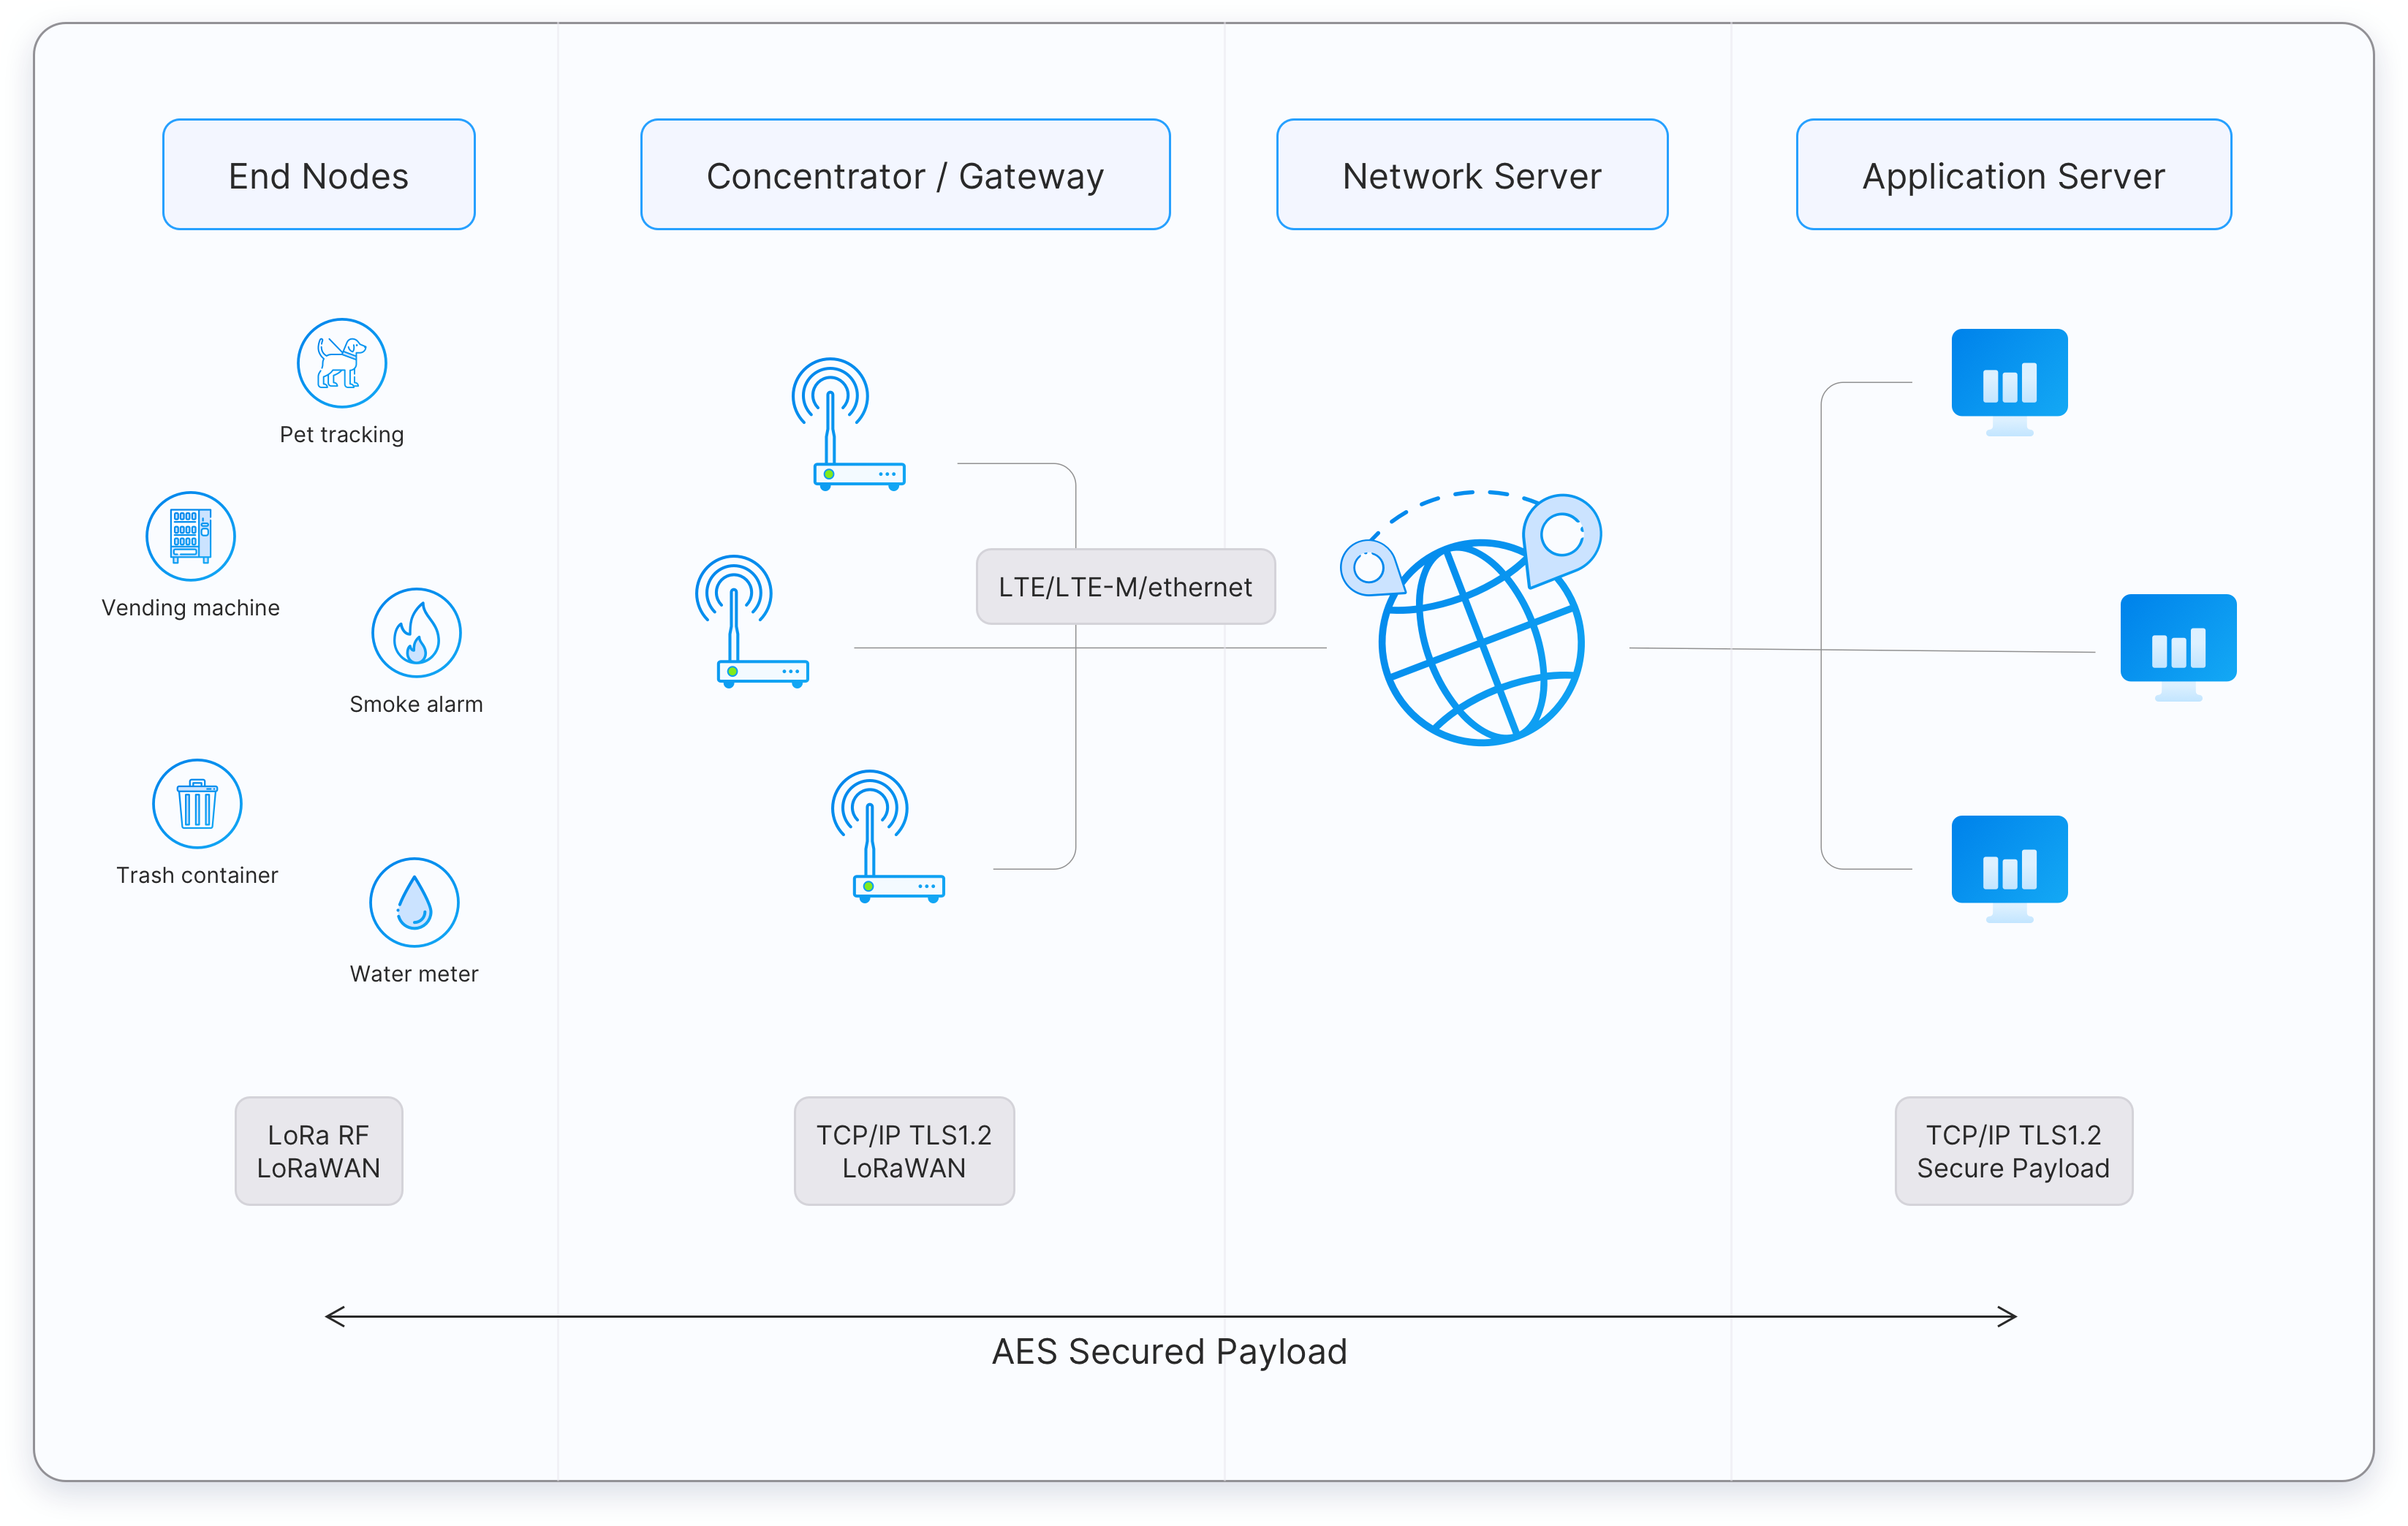
\includegraphics[width=1\textwidth]{pictures/lorawan-structure/lorawan-architecture.png}
    \caption{\ac{LoRaWAN} network structure~\protect\cite{the_things_network_lorawan_nodate}}\label{pic:lorawan-network-structure}
\end{figure}

\ac{LoRaWAN} uses the LoRa wireless communication protocol to create a \ac{WAN} where multiple devices can communicate with each other over long distances.

The \ac{LoRaWAN} network architecture, as seen in \cref{pic:lorawan-network-structure} consists of four main components~\cite[p. 8]{lora_alliance_inc_lorawan_2017}:

\begin{itemize}
    \item the end nodes (also called devices or motes),
    \item the gateways (also called concentrators or base stations),
    \item the \ac{LNS}, and
    \item the \acp{AS}.
\end{itemize}

\ac{LoRaWAN} data rates typically range from 0.3 kbps to 50 kbps, depending on the region and the \ac{LoRa} modulation used~\cite[p. 8]{lora_alliance_inc_lorawan_2017}.

\subsection{Data Transmission}

In LoRaWAN, data transmissions to and from the end nodes are called \emph{uplink} and \emph{downlink}, respectively~\cite[p. 12]{lora_alliance_inc_lorawan_2017}.

Uplinks are relayed to the network server by one or more gateways from the end node.
Downlinks, however, are only sent from the network server to the end node using a single gateway.
\subsection{Device Classes}

\ac{LoRaWAN} defines three classes of devices that offer different variations of the trade-off between power consumption and data rate/availability~\cite[p. 10]{lora_alliance_inc_lorawan_2017}.

\subsubsection{Class A}

\begin{figure}[h]
    \centering
    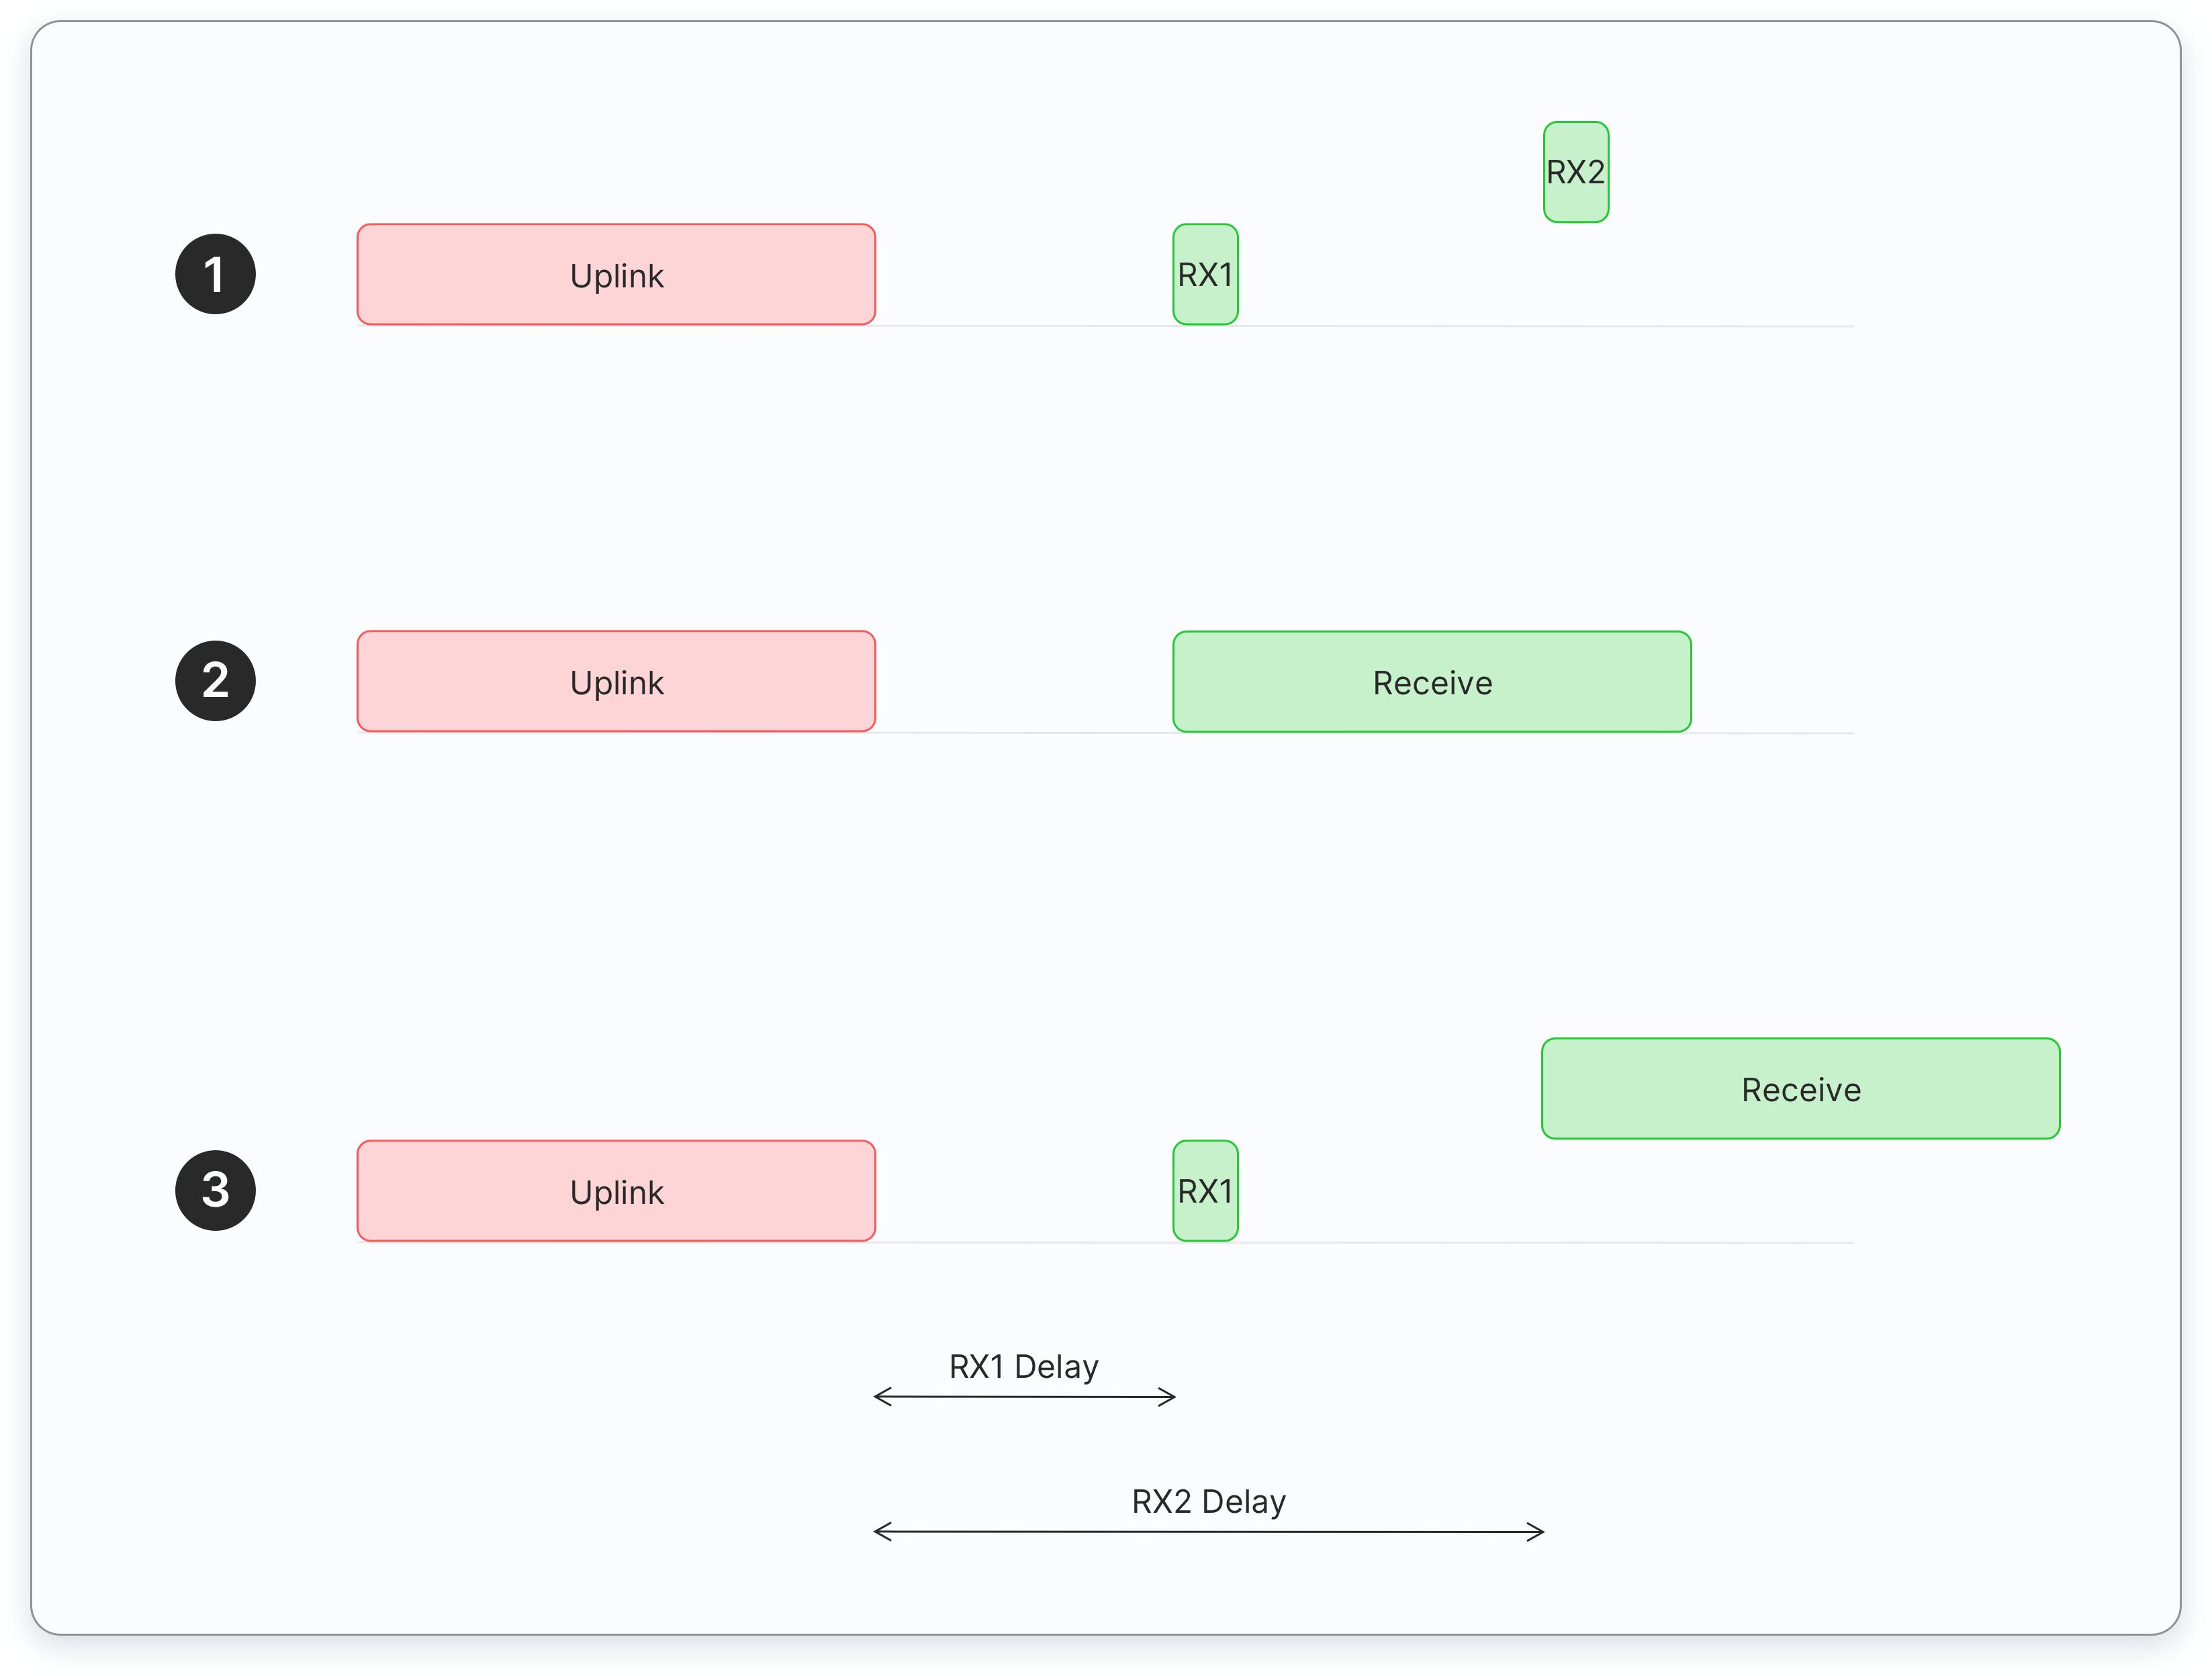
\includegraphics[width=0.9\textwidth]{pictures/device-classes/class-a.png}
    \caption{\ac{LoRaWAN} Device class A communication schema~\protect\cite{the_things_network_device_nodate}}\label{pic:lorawan-device-class-a-schema}
\end{figure}

Class A is used for devices that need to consume as little power as possible.
Every \ac{LoRaWAN} device must support the Class A mode~\cite[p. 11]{lora_alliance_inc_lorawan_2017}.
A communication in Class A is always initiated by the end device itself.

Bidirectional communication is possible in Class A through the use of two downlink receive windows during which it is possible for the \ac{LNS} to send data to the device.
This can be seen in \cref{pic:lorawan-device-class-a-schema}.
This also makes it impossible for the \ac{LNS} to send data to the device at any other time.

Class A consumes the least amount of power of the three classes, since the devices itself may specify when and how often they want to communicate with the \ac{LNS}.

\subsubsection{Class B}

\begin{figure}[h]
    \centering
    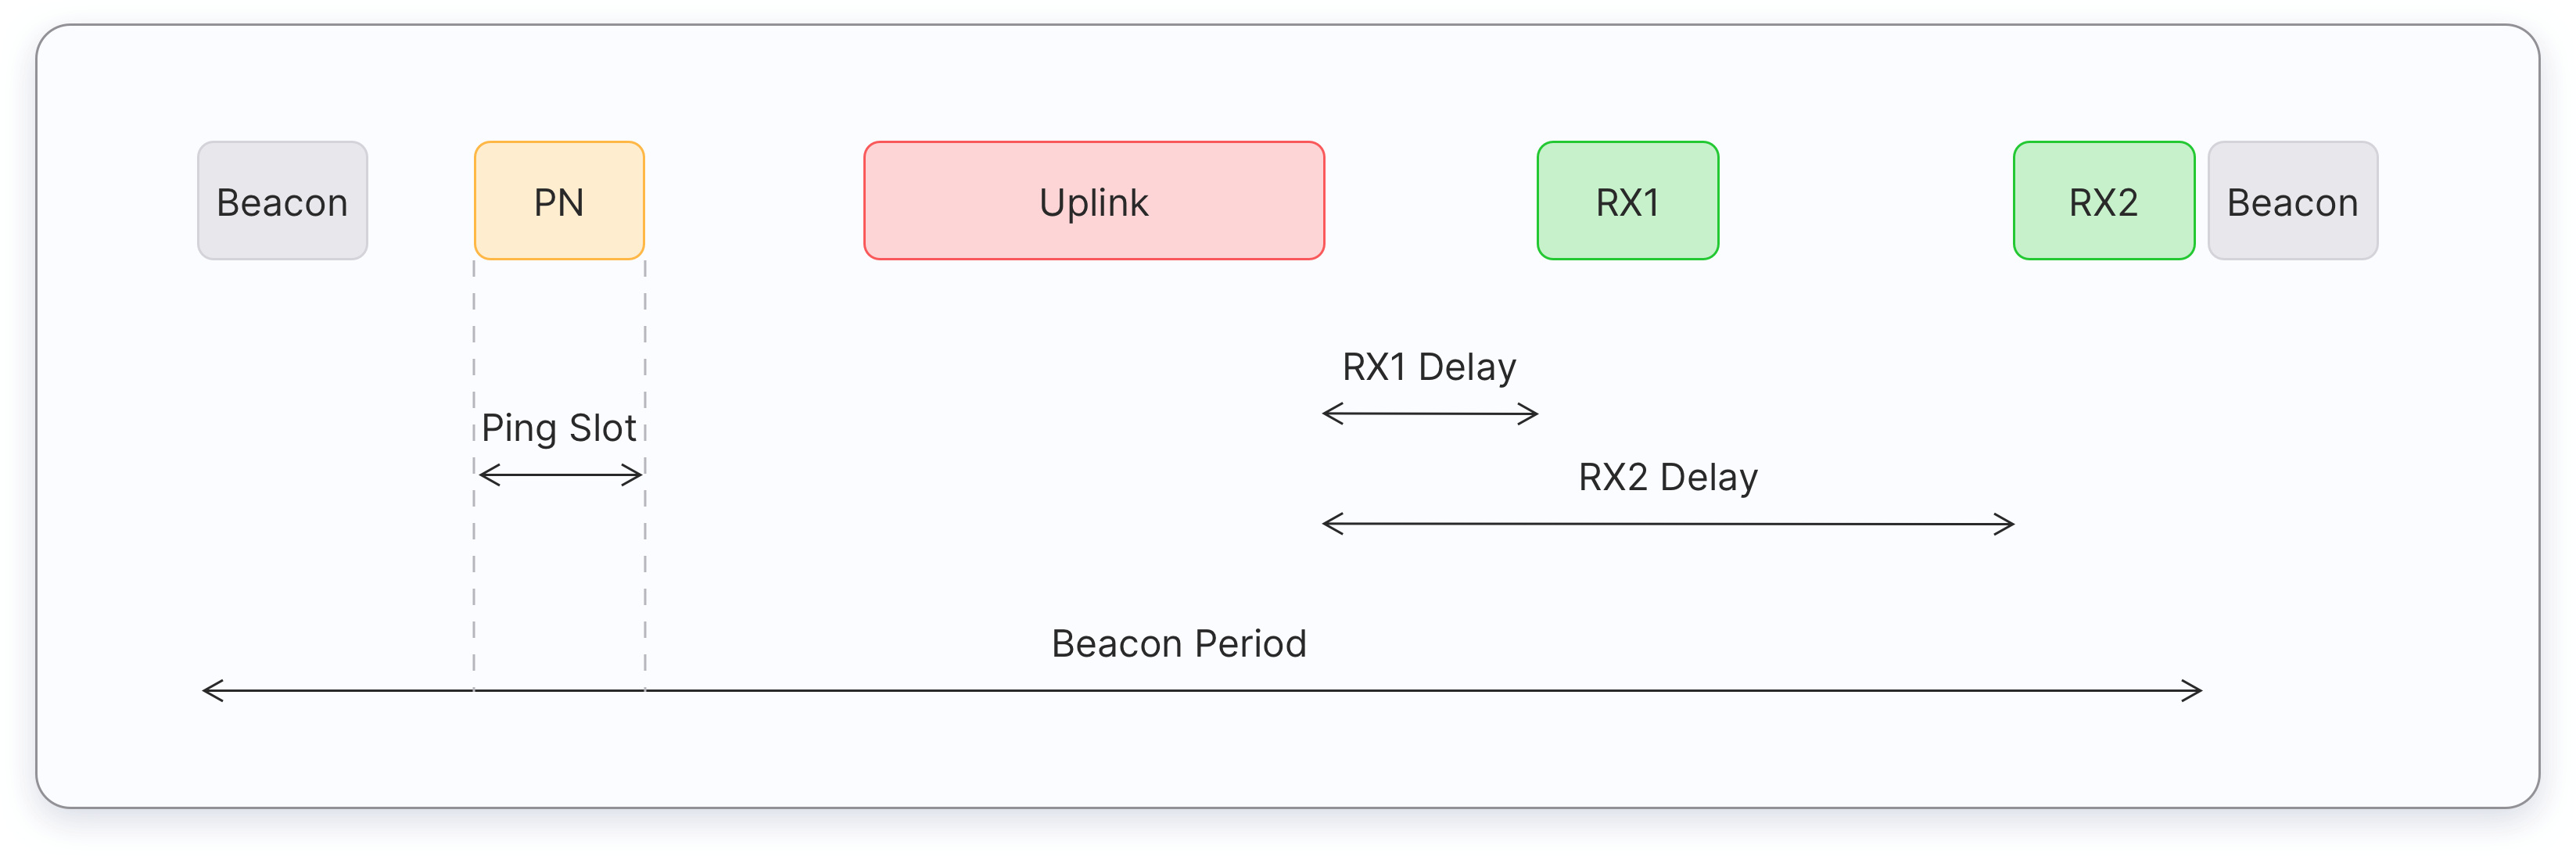
\includegraphics[width=0.9\textwidth]{pictures/device-classes/class-b.png}
    \caption{\ac{LoRaWAN} Device class B communication schema~\protect\cite{the_things_network_device_nodate}}\label{pic:lorawan-device-class-b-schema}
\end{figure}

In addition to class A, class B devices are also able to receive downlink messages from the \ac{LNS} during dedicated downlink receive windows.
In order to realize this without the need for a per-device \ac{RTC}, class B devices receive time synchronized beacons from the gateways.
The communication schema for class B devices can be seen in \cref{pic:lorawan-device-class-b-schema}.

These scheduled downlink windows result in a higher power consumption for class B devices, since those need to be awake during these windows.

\subsubsection{Class C}

\begin{figure}[h]
    \centering
    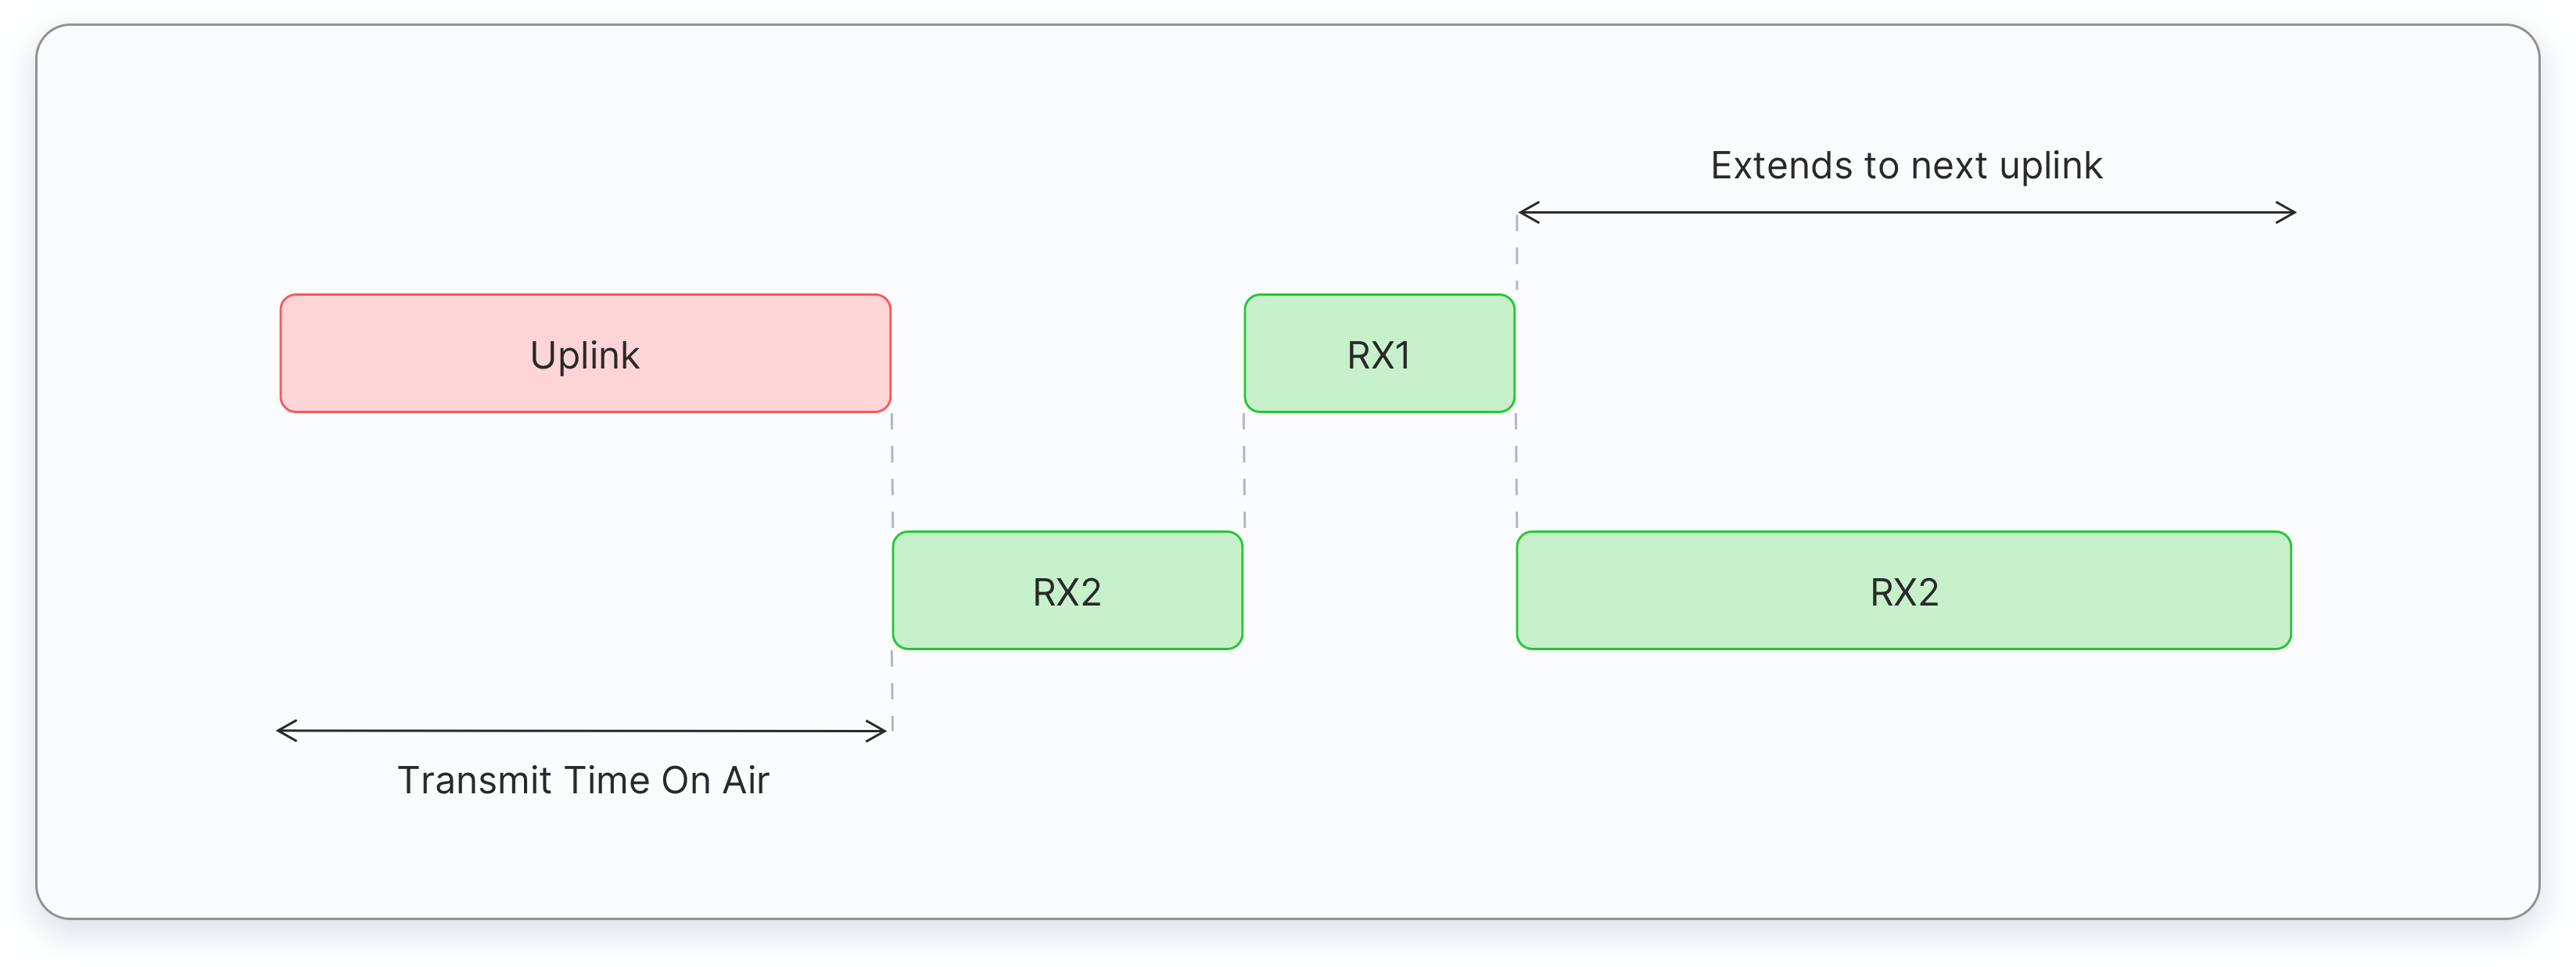
\includegraphics[width=0.9\textwidth]{pictures/device-classes/class-c.png}
    \caption{\ac{LoRaWAN} Device class C communication schema~\protect\cite{the_things_network_device_nodate}}\label{pic:lorawan-device-class-c-schema}
\end{figure}

Class C devices, when not currently transmitting an uplink message, are always listening for downlink messages from the \ac{LNS}.
In essence, they keep the downlink windows as specified in class B open all the time as seen in \cref{pic:lorawan-device-class-c-schema}.

Devices in class C consume the most power, since they are always listening for downlink messages.
The fact that they're always reachable by the \ac{LNS} also makes them the most suitable for applications that require a high data rate or a reliable accessibility via downlink.

\section{\acf{TTN}}

\ac{TTN} provides a free to use \ac{LNS} that supports a global community of people building \ac{LoRaWAN} applications.
It provides a free \ac{LoRaWAN} network for the public to use.

\ac{TTN} was used in this thesis to enable the communication between the \ac{LoRa} devices and TTNMapper.

\subsection{Gateways}

Gateways can forward \ac{LoRaWAN} packets that it receives to the \ac{LNS} in two major ways:

\subsubsection{\acf{SUPF}}

The \acl{SUPF} is a piece of software used to connect \ac{LoRa} gateways to the \ac{LNS}~\cite{the_things_network_semtech_nodate}.
The \ac{SUPF} relays \ac{LoRaWAN} packets that it receives from its connected \ac{LoRa} concentrator to the \ac{LNS} using the \ac{UDP} protocol.

It may be configured using JSON files such as \lstinline{global_conf.json} and \lstinline{local_conf.json}.

\subsubsection{\acf{LBS}}

Since \ac{TTN} v3, using the \ac{TCP}-based \acl{LBS} protocol is recommended over the \ac{SUPF} to connect gateways to the \ac{LNS}~\cite{the_things_network_semtech_nodate}.

\ac{LBS} uses TLS-encrypted \ac{TCP} connections with token-based authentication to relay \ac{LoRaWAN} packets to the \ac{LNS}~\cite{the_things_network_lora_nodate}.

The two main components of \acl{LBS} are the \ac{LNS} itself as well as the \acf{CUPS}.

While the \ac{LNS} is responsible for handling the \ac{LoRaWAN} packets, the \acl{CUPS} is responsible for handling the configuration of the gateways.

While \ac{CUPS} is not strictly necessary for sending actual \ac{LoRaWAN} packets, it simplifies the management of gateways and their configuration.
When a gateway is configured with \ac{CUPS}, it will automatically receive its configuration from the \ac{LNS} and be authenticated to work with it~\cite{the_things_network_lora_nodate}.

\section{Localization of devices}

\subsection{Technologies}

\subsubsection{\ac{GPS}}

% Genauigkeit von GPS mit quelle
% GPS verwendet lateration -> quelle

\subsection{Triangulation}

\subsection{Multilateration}

\subsection{\acs{ToA}-based}

The \acf{ToA} based method uses the difference in the signal's time of arrival at the receiving stations.
In conjunction with the speed of light, this time difference can be used to calculate the distance between the receiving stations and the transmitting station.

\ac{ToA} is being used by radio location systems like \ac{GPS} to determine the position of a device by using Multilateration.

\subsection{\acs{TDoA}-based}

% how does it work

\subsection{\acs{RSSI}-based}

The method based on \acf{RSSI} uses the signal strength of the signal that is received.
Since signal strengths are not linear, the \ac{RSSI} values need to be converted to a linear scale.
Different devices can have different \ac{RSSI} values for the same distance.
\ac{RSSI} values can only function reliably when there is nothing blocking the signal between the transmitting and receiving stations, e.g. if there is a line of sight between the sender and receiver.

% does this belong here or in the implementation chapter?
\section{Used \ac{LoRa} Hardware}

\subsection{Gateways}

% list the gateways that were used, images

% Mikrotik lr8 + antenne (deployment on ask, ghb)
% Dragino LG308 (deployment c building)

\subsection{Nodes}

% list the nodes that were used

% HTCC-AB02s
% ELV GPS long boi
% dnt solar tracker

\section{\acf{TTNM}}

% TODO explain who made it and when

% explain how it works in conjunction with TTN

% explain why it is important for the thesis